%%==================================================================%%
%% Author : Tejedo Gonz�lez, Daniel                                 %%
%%          S�nchez Barreiro, Pablo                                 %%
%% Version: 1.0, 18/11/2012                                         %%                   %%                                                                  %%
%% Memoria del Proyecto Fin de Carrera                              %%
%% Antecedentes, archivo ra�z                                       %%
%%==================================================================%%

\chapterheader{Antecedentes}{Antecedentes}
\label{chap:background}

Este cap�tulo trata de describir a grandes rasgos las t�cnicas, tecnolog�as y herramientas utilizadas para el desarrollo del presente Proyecto Fin de Carrera. En primer lugar, se introducir� el caso de estudio que se utilizar� de forma recurrente a lo largo del proyecto, que es una l�nea de productos software para software de control para hogares inteligentes. Para ello se describen en primer lugar diversos conceptos relacionados el dominio del proyecto, como son las l�neas de productos software y los �rboles de caracter�sticas. A continuaci�n, se describen dos principales herramientas de Ingenier�a de Lenguajes Dirigida por Modelos utilizadas: \emph{Ecore} y \emph{EMFText}. Por �ltimo, se describe brevemente la arquitectura de plugins de Eclipse, dado que nuestro proyecto deb�a integrarse en dicho entorno.

\chaptertoc

\section{Caso de Estudio: Software para Hogares Inteligentes}
\label{sec:back:spl}
%%==================================================================%%
%% Author : Abascal Fern�ndez, Patricia                             %%
%%          S�nchez Barreiro, Pablo                                 %%
%% Version: 1.1, 17/04/2013                                         %%
%%                                                                  %%
%% Memoria del Proyecto Fin de Carrera                              %%
%% Planificacion/CasoEstudio                                        %%
%%==================================================================%%

El objetivo �ltimo del presente proyecto es la construcci�n de una l�nea de productos software sobre la plataforma .NET para hogares automatizados y/o inteligentes.

El objetivo de estos hogares es aumentar la comodidad y seguridad de sus habitantes, as� como hacer un uso m�s eficiente de la energ�a consumida. Los ejemplos m�s comunes de tareas automatizadas dentro de un hogar inteligente son el control de las luces, ventanas, puertas, persianas, aparatos de fr�o/calor, as� como otros dispositivos, que forman parte de un hogar. Un hogar inteligente tambi�n busca incrementar la seguridad de sus habitantes mediante sistemas automatizados de vigilancia y alerta de potenciales situaciones de riesgo. Por ejemplo, el sistema deber�a encargarse de detecci�n de humos o de la existencia de ventanas abiertas cuando se abandona el hogar.

El funcionamiento de un hogar inteligente se basa en el siguiente esquema: (1) el sistema lee datos o recibe datos de una serie de sensores; (2) se procesan dichos datos; y (3) se activan los actuadores para realizar las  acciones que correspondan en funci�n de los datos recibidos de los sensores.

Todos los sensores y actuadores se comunican a trav�s de un dispositivo especial denominado puerta de enlace (\emph{Gateway}, en ingl�s). Dicho dispositivo se encarga de coordinar de forma adecuada los diferentes dispositivos existentes en el hogar, de acuerdo a los par�metros y preferencias especificados por los habitantes del mismo. Los habitantes del hogar se comunicar�n con la puerta de enlace a trav�s de una interfaz gr�fica.
Este proyecto tiene como objetivo el desarrollo de un hogar inteligente como una l�nea de productos software, con un n�mero variable de plantas y habitaciones. El n�mero de habitaciones por planta es tambi�n variable. La l�nea de productos deber� ofrecer varios servicios, que podr�n ser opcionalmente incluidos en la instalaci�n del software para un un hogar determinado. Dichos servicios se clasifican en funciones b�sicas y complejas, las cuales describimos a continuaci�n.

\paragraph{Funciones b�sicas} \ \\

\begin{enumerate}
\item \emph{Control autom�tico de luces:} Los habitantes del hogar deben ser capaces de encender, apagar y ajustar la intensidad de las diferentes luces de la casa. El n�mero de luces por habitaci�n es variable. El ajuste debe realizarse especificando un valor de intensidad.
\item \emph{Control autom�tico de ventanas:} Los residentes tienen que ser capaces de controlar las ventanas autom�ticamente. De tal modo que puedan indicar la apertura de una ventana desde las interfaces de usuario disponibles.
\item \emph{Control autom�tico de persianas:} Los habitantes podr�n subir y bajar las persianas de las ventanas de manera autom�tica.
\item \emph{Control autom�tico de temperatura:} El usuario ser� capaz de ajustar la temperatura de la casa. La temperatura se medir� siempre en grados celsius.
\end{enumerate}

\paragraph{Funciones complejas} \ \\

\begin{enumerate}
\item \emph{Control inteligente de energ�a:} Esta funcionalidad trata de coordinar el uso de ventanas y aparatos de fr�o/calor para regular la temperatura interna de la casa de manera que se haga un uso m�s eficiente de la energ�a. Por ejemplo, si se recibe la orden de calentar la casa, a la vez que se activan los radiadores se cerrar�n las ventanas para evitar las p�rdidas de calor.
\item \emph{Presencia simulada:} Para evitar posibles robos, cuando los habitantes abandonen la casa por un periodo largo de tiempo, se deber� poder simular la presencia de personas en las casas. Hay dos opciones de simulaci�n (no exclusivas):
	\begin{enumerate}
	\item \emph{Simulaci�n de las luces:} Las luces se deber�n apagar y encender para simular la presencia de habitantes en la casa.
	\item \emph{Simulaci�n de persianas:} Las persianas se deber�n subir y bajar autom�tica para simular la presencia de individuos dentro de la casa.
	\end{enumerate}
\end{enumerate}

Todas estas funciones son opcionales. Las personas interesadas en adquirir el sistema podr�n incluir en una instalaci�n concreta de este software el n�mero de funciones que ellos deseen. La siguiente secci�n profundiza en el concepto \emph{l�nea de productos software}. 

\section{L�neas de producto software}
\label{sec:back:spl}
%%==================================================================%%
%% Author : Abascal Fern�ndez, Patricia                             %%
%%          S�nchez Barreiro, Pablo                                 %%
%% Version: 1.3, 18/06/2013                                         %%
%%                                                                  %%
%% Memoria del Proyecto Fin de Carrera                              %%
%% Background/Software Product Lines                                %%
%===================================================================%%

El objetivo de una \emph{l�nea de producto software}~\citep{pohl:2010,kakola:2006} es crear una infraestructura adecuada a partir de la cual se puedan derivar, de forma tan autom�tica como sea posible, producto concretos pertenecientes a una familia de producto software. Una familia de producto software es un conjunto de aplicaciones software similares, lo que implica que comparten una serie de caracter�sticas comunes, pero que tambi�n presentan variaciones entre ellos.

Un ejemplo cl�sico de familia de producto software es el producto Parten�n, para software bancario, comentado en la introducci�n a este documento (ver Secci�n~\ref{sec:intr:introduction}). Dicho producto representa una familia de productos destinados a la gesti�n bancaria. Parten�n en s� no puede ser desplegado como una aplicaci�n, sino que necesita ser configurado de acuerdo a una serie de caracter�sticas concretas demandadas por cada cliente que require una instalaci�n de Parten�n.

La idea de una l�nea de producto software es proporcionar una forma autom�tica y sistem�tica de construir productos concretos dentro de una familia de producto software mediante la simple especificaci�n de qu� caracter�sticas deseamos incluir dentro de dicho producto. Esto representa una alternativa al enfoque tradicional de desarrollo software, el cual se basaba simplemente en seleccionar el producto m�s parecido, dentro de la familia, al que queremos construir y adaptarlo manualmente.

El proceso de creaci�n de l�neas de producto software se estructura dos fases: (1) \emph{Ingenier�a del Dominio} (en ingl�s,  \emph{Domain Engineering}); y (2) \emph{Ingenier�a de Aplicaci�n} (en ingl�s, \emph{Application Engineering}) (ver Figura~\ref{back:fig:domainAplicEng}). La \emph{Ingenier�a del Dominio} tiene como objetivo la creaci�n de la infraestructura o arquitectura de referencia de la l�nea de productos software. Esta arquitectura de referencia debe permitir la r�pida, o incluso autom�tica, construcci�n de sistemas software espec�ficos pertenecientes a la familia de productos software. La \emph{Ingenier�a de Aplicaci�n} utiliza la infraestructura creada anteriormente para crear aplicaciones espec�ficas adaptadas a las necesidades de cada usuario en concreto.

\begin{figure}[!tb]
  \centering
  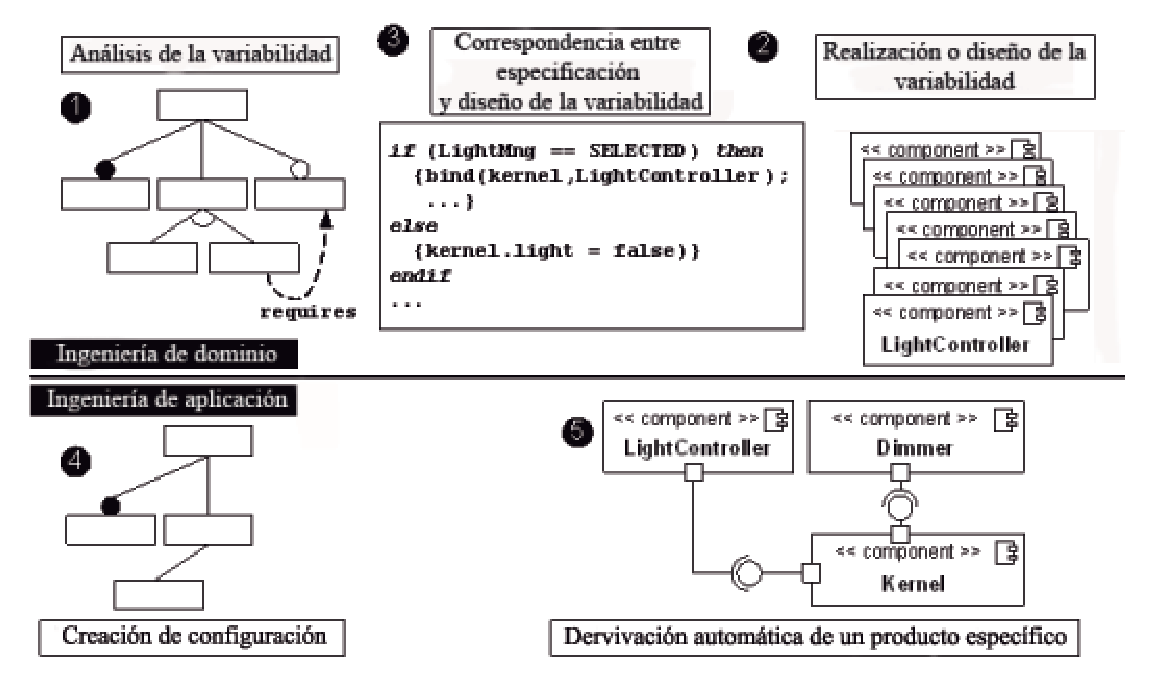
\includegraphics[width=.95\linewidth]{background/images/domainAplicationEngineering.eps} \\
  \caption{Proceso de Desarrollo de una l�nea de producto software}
  \label{back:fig:domainAplicEng}
\end{figure}

En la fase de Ingenier�a del Dominio, el primer paso a realizar es un an�lisis de qu� caracter�sticas de la familia de producto son variables y por qu� son variables. Esta parte es la que se conoce como \emph{An�lisis o Especificaci�n de la Variabilidad} (Figura~\ref{back:fig:domainAplicEng}, etiqueta 1).

A continuaci�n, se ha de dise�ar una arquitectura de referencia para la familia de producto software que permita soportar dicha variabilidad. Esta actividad se conoce como \emph{Realizaci�n o Dise�o de la Variabilidad} (Figura~\ref{back:fig:domainAplicEng}, etiqueta 2).

El siguiente paso es establecer una serie de reglas que especifiquen c�mo hay que instanciar o configurar la arquitectura previamente creada de acuerdo con las caracter�sticas seleccionadas por cada cliente. Esta fase es la que se conoce como \emph{Correspondencia entre Especificaci�n y Dise�o de la Variabilidad} (Figura~\ref{back:fig:domainAplicEng}, etiqueta 3).

Tras completar la fase de Ingenier�a del Dominio, disponemos de una especie de l�nea de montaje, la cual podemos utilizar para construir productos concretos de forma m�s o menos automatizada.

En la fase de Ingenier�a de Aplicaci�n, se crean productos concretos utilizando la infraestructura previamente creada. Para ello, el primer paso es crear una \emph{configuraci�n}, que no es m�s que una selecci�n de caracter�sticas que un usuario desea incluir en su producto concereto (Figura~\ref{back:fig:domainAplicEng}, etiqueta 4).

En el caso ideal, usando esta configuraci�n, se debe poder ejecutar las reglas de correspondencia entre especificaci�n y dise�o de la variabilidad para que la arquitectura creada en la fase de Ingenier�a del Dominio se adapte autom�ticamente; generando un producto concreto espec�fico acorde a las necesidades concretas del usuario (Figura~\ref{back:fig:domainAplicEng}, etiqueta 5). En el caso no ideal, dichas reglas de correspondencia deber�n ejecutarse a mano, lo cual suele ser un proceso tedioso, largo, repetitivo y propenso a errores.

La siguiente secci�n describe el paradigma de desarrollo software orientada a caracter�sticas, el cual est� �ntimamente ligado al dise�o e implementaci�n de l�neas de productos software.



\section{�rboles de caracter�sticas}
\label{sec:back:fmodels}
%%==================================================================%%
%% Author : Tejedo Gonz�lez, Daniel                                 %%
%%          S�nchez Barreiro, Pablo                                 %%
%% Version: 1.0, 18/11/2012                                         %%                   
%% Version: 2.0, 05/02/2013                                         %%                   
%%                                                                  %%
%% Memoria del Proyecto Fin de Carrera                              %%
%% Antecedentes, �rboles de caracter�sticas                         %%
%%==================================================================%%

Como se ha comentado en la secci�n anterior, una de las tareas clave para el �xito de una l�nea de productos software consiste en analizar la variabilidad existente en la familia de productos software que dicha l�nea de productos software pretende cubrir. Aqu� es donde entran en juego los \emph{�rboles de caracter�sticas}~\cite{}. Una \emph{caracter�stica} se define como ''\emph{un incremento en la funcionalidad del producto}'', o m�s formalmente, ''\emph{una caracter�stica es una propiedad de un sistema que es relevante a algunos \emph{stakeholders} y que es utilizada para capturar propiedades comunes o diferenciar entre sistemas de una misma familia}"~\cite{}. De este modo un producto queda representado por las caracter�sticas que posee.

Para poder capturar las divergencias y aspectos comunes entre los distintos productos de una misma familia, los �rboles de caracter�sticas organizan de forma jer�rquica el conjunto de caracter�sticas que posee una familia de productos. Cada caracter�stica se representa como un nodo ene la �rbol de caracter�sticas. La ra�z de dicho �rbol es siempre el sistema o producto software cuya variabilidad estamos analizando. Cada caracter�stica se puede descomponer en varias subcaracter�sticas, siendo est�s �ltimas nodos \emph{hijos} de la primera caracter�sticas, que actuar�a como \emph{padre}. Dependiendo de sis dichas subcaracter�sticas son obligatorias, alternativas u opcionales, existen diversos tipos de relaciones padre-hijo. 

%%=========================================================================================%%
%% NOTA(Pablo): Para esta figura, hazte un modelo para la Smart Home sin habitaciones ni   %%
%%              plantas. Lo puedes encontrar en un art�culo que te mando luego             %% %%=========================================================================================%%
\begin{figure}[!tb]
    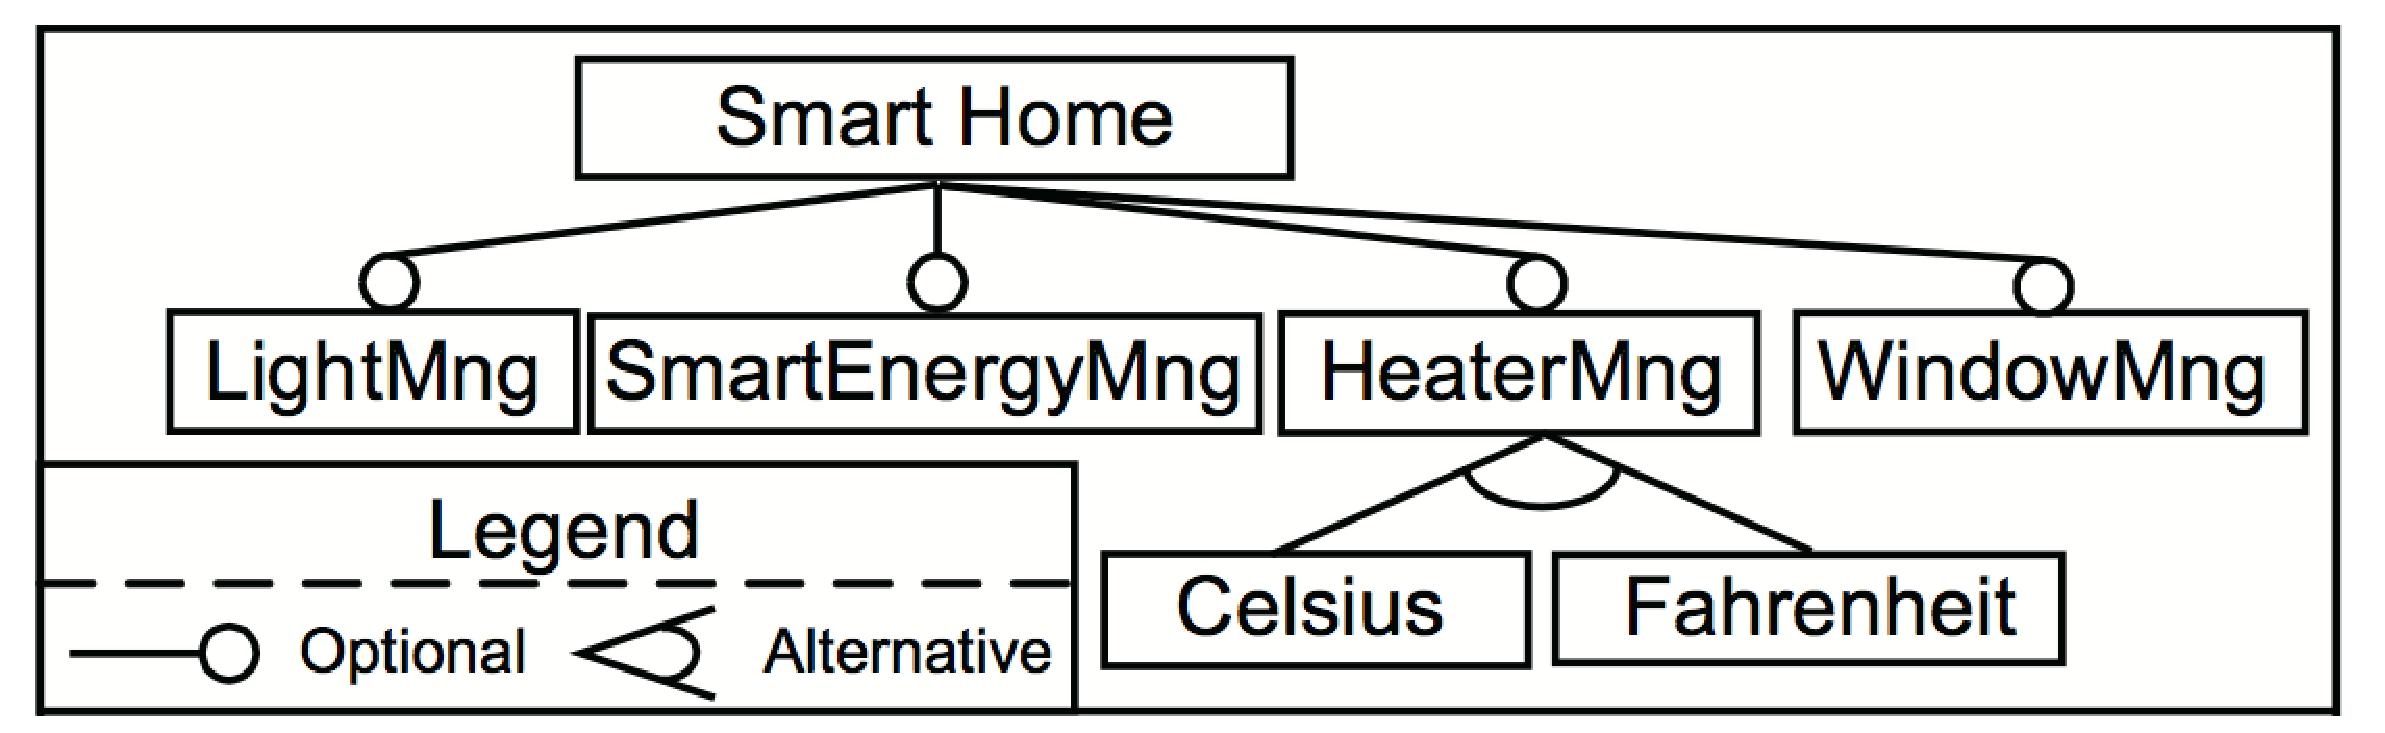
\includegraphics[scale=0.3]{background/simpleSmarthome.eps}
    \caption{�rbol de caracter�sticas simple para nuestro caso de estudio}
    \label{fig:smartHomeFMsimple}
\end{figure}

La Figura~\ref{fig:smartHomeFMsimple} muestra como ejemplo un �rbol de caracter�sticas que especifica la variabilidad inherente a nuestro caso de estudio, sin considerar que las plantas y habitaciones puedan configurarse de manera individual. El �rbol representa un hogar inteligente definido por las siguientes caracter�sticas: controlador de luz, controlador de temperatura, controlador de ventanas y controlador de la energ�a. Tal como se puede ver en la leyenda de la figura, todas estas caracter�sticas son opcionales, es decir, podemos decidir si queremos que est�n o no presentes en el hogar inteligente que generemos. Adem�s, para la caracter�stica ''controlador de temperatura" se ha de especificar una de las dos opciones alternativas que se plantean: grados celsius o grados fahrenheit.

El modo de representaci�n de los �rboles de caracter�sticas permite especificar cierto tipo de restricciones que pueden resultar necesarias para representar con exactitud el comportamiento del producto que queramos construir. En el caso de la Figura~\ref{fig:smartHomeFMsimple} se puede observar que mediante las relaciones ya se est� modelando la restricci�n que especifica que el controlador de temperatura ha de ser necesariamente de uno de los tipos que se indican en el modelo. Otros tipos de relaciones que pueden incluirse sirven para especificar otras restricciones, por ejemplo la obligatoriedad de seleccionar una caracter�stica o un grupo de ellas.

Sin embargo, si quisi�ramos incluir algunas restricciones m�s complejas, la representaci�n gr�fica de los �rboles de caracter�sticas se queda corta. Por ejemplo, en la Figura~\ref{fig:smartHomeFMsimple} podr�amos querer especificar la restricci�n de que si nuestro hogar inteligente tiene un controlador de energ�a, ha de tener tambi�n un controlador de calefacci�n en grados celsius. Es imposible modelar esta restricci�n con las herramientas de las que los �rboles de caracter�sticas disponen. Es por ese motivo que debe permitirse la posibilidad de especificar restricciones externas al �rbol mediante alg�n tipo de lenguaje textual o gr�fico.

%%=========================================================================================%%
%% NOTA(Pablo): Explicar el modelo creado, indicando las cosas que son variables, las que  %%
%%              son alternativas, etc.                                                     %%
%%              Explicar el problema de las restricciones externas                         %%
%%=========================================================================================%%

\begin{figure}[!tb]
    \centerline{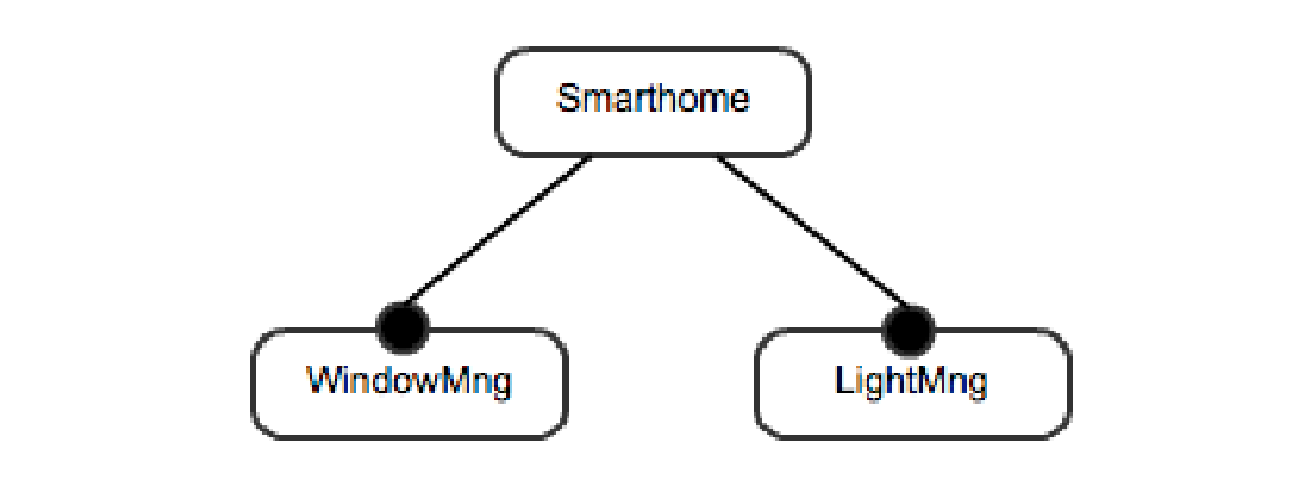
\includegraphics[scale=0.3]{background/simpleSmarthomeConf.eps}}
    \caption{Configuraci�n para la versi�n sencilla del caso de estudio}
    \label{fig:smartHomeConfSimple}
\end{figure}

Una vez creado un �rbol de caracter�sticas para una l�nea de productos software, podemos indicar las caracter�sticas que podemos incluir en un producto software concreto mediante la creaci�n de configuraciones. Una \emph{configuraci�n} no es m�s que una selecci�n v�lida de caracter�sticas. La Figura~\ref{fig:smartHomeConfSimple} muestra en un ejemplo de configuraci�n para el modelo de la Figura~\ref{fig:smartHomeFMsimple} donde se indica que el producto que deseamos construir debe incluir �nica y obligatoriamente un dispositivo de control de luz y un dispositivo de control de ventanas. Obviamente, dicho modelo debe satisfacer las restricciones externas declaradas. 

Los �rboles de caracter�sticas como los anteriormente expuestos no permiten modelar que pueda existir un n�mero variable de ciertas caracter�sticas, como, en nuestro caso, de plantas y habitaciones, y que, adem�s, cada instancia particular de una caracter�sticas pueda  configurarse de forma distinta. Por ejemplo, podr�amos decidir que el sal�n de la casa tenga control inteligente de temperatura, mientras que la cocina, que est� sometida a mayores variaciones de temperatura, no contenga dicha caracter�sticas. Para solventar esta carencia, se introdujeron en los �rboles de caracter�sticas el concepto de caracter�stica clonable. 

\begin{figure}[!tb]
    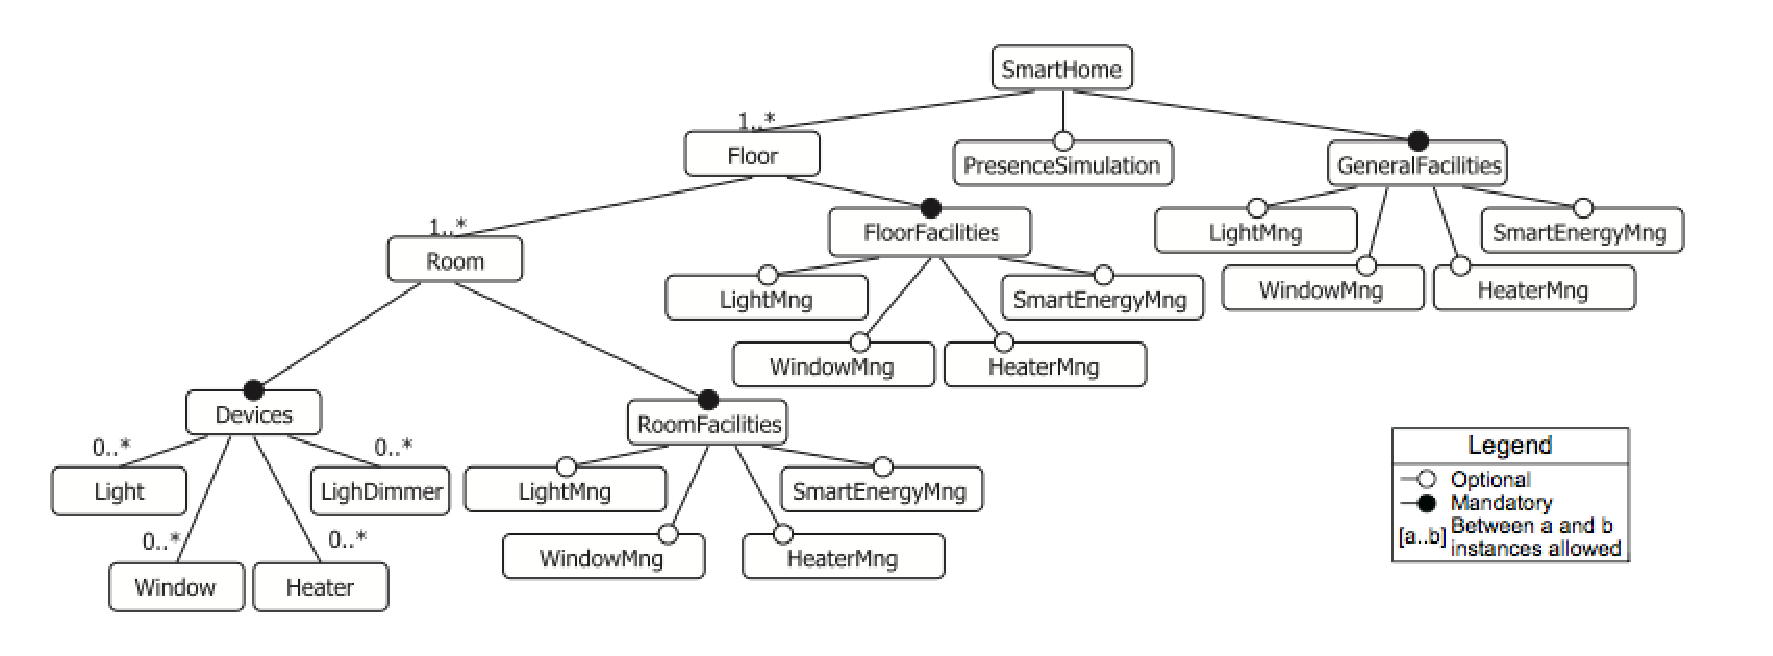
\includegraphics[scale=0.4]{background/featuremodel.eps}
    \caption{�rbol de caracter�sticas completo para nuestro caso de estudio}
    \label{fig:smarHomeFeatureModel}
\end{figure}

La Figura~\ref{fig:smarHomeFeatureModel} muestra el �rbol de caracter�sticas para nuestro caso de estudio incluyendo \emph{caracter�sticas clonables}. Las caracter�sticas Floor (Piso) y Room (Habitaci�n) son clonables porque pueden aparecer m�s de una vez en las configuraciones creadas. La cardinalidad de ambas caracter�sticas es 1..*, lo que significa que pueden ser seleccionadas de una a infinitas veces. As� mismo, cualquier caracter�stica que sea hija de ellas directa o indirectamente es considerada inmediatamente como caracter�stica. Este es el caso, por ejemplo, de Devices y de sus caracter�sticas hijas (Heater, Window, etc.), que son consideradas clonables tanto por su cardinalidad como por ser hijas de una caracter�stica clonable. 

La repetici�n de las caracter�sticas correspondientes a los diversos controladores (es decir, WindowMng, HeaterMng, etc.) se debe a que gracias a las caracter�sticas clonables ahora podemos diferenciar los controladores seg�n su colocaci�n y alcance. Es decir, el controlador de temperatura hijo de RoomFacilities afectar� s�lo a la habitaci�n a la que pertenezca, el hijo de FloorFacilities afectar� al piso al que pertenezca, y el hijo de GeneralFacilities afectar� a todo el hogar creado. 
%%=========================================================================================%%
%% NOTA(Pablo): A�adir la figura, si no te entrase bien a lo ancho, mira como meterla 
%%              apaisada en Latex.
%%=========================================================================================%%

A la hora de crear configuraciones para este nuevo �rbol hay que tener en cuenta que podemos seleccionar en m�s de una ocasi�n ciertas caracter�sticas, por lo que necesitamos valernos de alg�n mecanismo que nos permita diferenciarlas entre ellas. El modo de lograrno es poniendo un nombre a las diferentes selecciones que hagamos de una misma caracter�stica. 

La Figura~\ref{fig:smarthomeCompleteConf} muestra un ejemplo de configuraci�n para el �rbol de caracter�sticas con caracter�sticas clonables de la Figura~\ref{fig:smarHomeFeatureModel}. En ella se puede apreciar que se diferencia entre las diferentes selecciones de la caracter�stica Floor poni�ndoles un nombre, en este caso Ground (Planta Baja) y First (Primer Piso). Del mismo modo con las habitaciones Kitchen (Cocina) y Living (Sal�n), pertenecientes a la planta baja, y Bed (Dormitorio), perteneciente al primer piso. Observando el �rbol de la figura es sencillo comprender qu� elementos y/o controladores tiene instalados cada estancia. Por ejemplo, la cocina est� dotada de dos luces, un regulador de luz, una ventana, un controlador de luz y un controlador de ventanas.

%%=========================================================================================%%
%% NOTA(Pablo): Explicar como se configuran las caracter�sticas clonables usando un 
%%              ejemplo
%%=========================================================================================%%

Como en el caso anterior, las diversas configuraciones no s�lo han de cumplir las restricciones impuestas por el propio �rbol de caracter�sticas, sino tambi�n las restricciones externas. Pero debido a la presencia de caracter�sticas clonables ahora existe una posibilidad mucho mayor de restricciones posibles que definir. Del mismo modo que antes se pod�an definir diversas restricciones l�gicas (a implies b), la presencia de caracter�sticas clonables hace que tambi�n sean necesarias las restricciones num�ricas (a >= b), lo que tambi�n a�ade la dificultad de diferenciar cuales caracter�sticas pueden realizar operaciones l�gicas y cuales no . 

Tambi�n es necesaria una operaci�n de contexto que permita aplicar estas restricciones s�lamente a sub�rboles de la configuraci�n. Esto es imprescindible para definir una restricci�n que, por ejemplo, valide que si una habitaci�n tiene un controlador de ventanas forzosamente ha de tener instalada al menos una ventana. Sin la operaci�n de contexto ser�a imposible saber a qu� caracter�stica WindowMng en concreto est� haciendo referencia la restricci�n definida.

El objetivo de este proyecto es implementar un lenguaje textual que haga posible la definici�n de restricciones externas para �rboles de caracter�sticas con caracter�sticas clonables con todas las peculiaridades definidas anteriormente, as� como una herramienta que permita validar si las configuraciones creadas satisfacen o no esas restricciones. 
%%=========================================================================================%%
%% NOTA(Pablo): Explicar el problema de las restricciones cuando incluyen caracter�sticas
%%              clonables y decir que implementar un lenguaje para resolver ese problema 
%%              es el objetivo de este proyecto
%%=========================================================================================%%

%%=========================================================================================%%
%% NOTA(Pablo): Esto no se entiende de forma clara, por lo que se suprime                                         %%
%%=========================================================================================%%
%%
%% Por otro lado, un modelo de caracter�sticas debe poder representar la cardinalidad de 
%% las caracter�sticas, por motivos tanto de comprensi�n (es mucho mejor contar con un 
%% �rbol de 8 nodos que con uno de 100, teniendo ambos un significado equivalente), como 
%% de funcionalidad, ya que permite expresar ciertas restricciones que de no contar con 
%% la cardinalidad no podr�an expresarse.
%% 
%% Adem�s se podr�n disponer de restricciones de usuario m�s complejas, que son las que
%% se han implementado en el editor de especificaci�n y validaci�n de restricciones 
%% desarrollado en este proyecto.
%%
%%=========================================================================================%%

%%=========================================================================================%%
%% NOTA(Pablo): Esto queda obsoleto en el nuevo esquema, por lo cual se suprime            %%
%%=========================================================================================%%
%%
%% La figura \ref{fig7} muestra un ejemplo de modelo de caracter�sticas. En este caso se 
%% trata de un modelo de una casa inteligente o SmartHome, a trav�s del cual, 
%% seleccionando ciertas caracter�sticas u otras podremos construir qu� tipo de casa 
%% queremos. Cada una de las m�ltiples casas diferentes que podamos construir es lo que 
%% se denonima una especializaci�n o configuraci�n de nuestro modelo de caracter�sticas.
%% 
%%  El proceso de crear una configuraci�n a partir de un modelo de caracter�sticas se 
%% conoce como proceso de configuraci�n o proceso de especializaci�n. Consiste en 
%% transformar un modelo de caracter�sticas de tal forma que el modelo resultante sea un
%%  subconjunto de las posibles configuraciones denotadas por el primer modelo. La figura 
%% \ref{fig8} muestra una posible configuraci�n para el modelo de caracter�sticas de la figura %% \ref{fig7}.
%%
%% La relaci�n entre un diagrama de caracter�sticas y una configuraci�n es an�loga a la
%% existenteentre una clase y una de sus instancias en programaci�n orientada a objetos.
%%
%%=========================================================================================%%

\begin{figure}[!tb]
    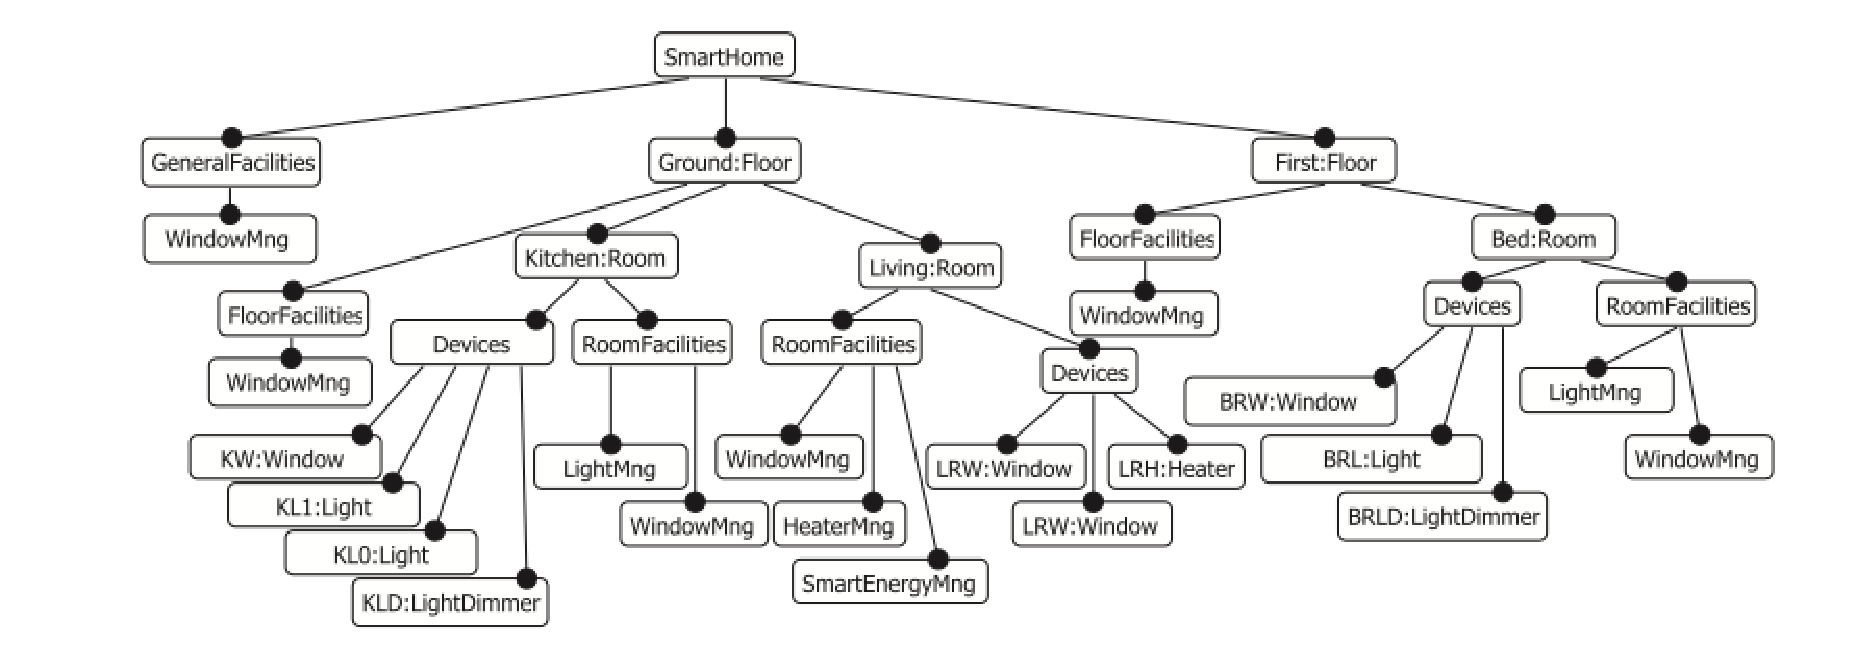
\includegraphics[scale=0.4]{background/configuration.eps}
    \caption{Posible modelo de configuraci�n de una casa inteligente concreta}
    \label{fig:smarthomeCompleteConf}
\end{figure}

\begin{figure}[!tb]
    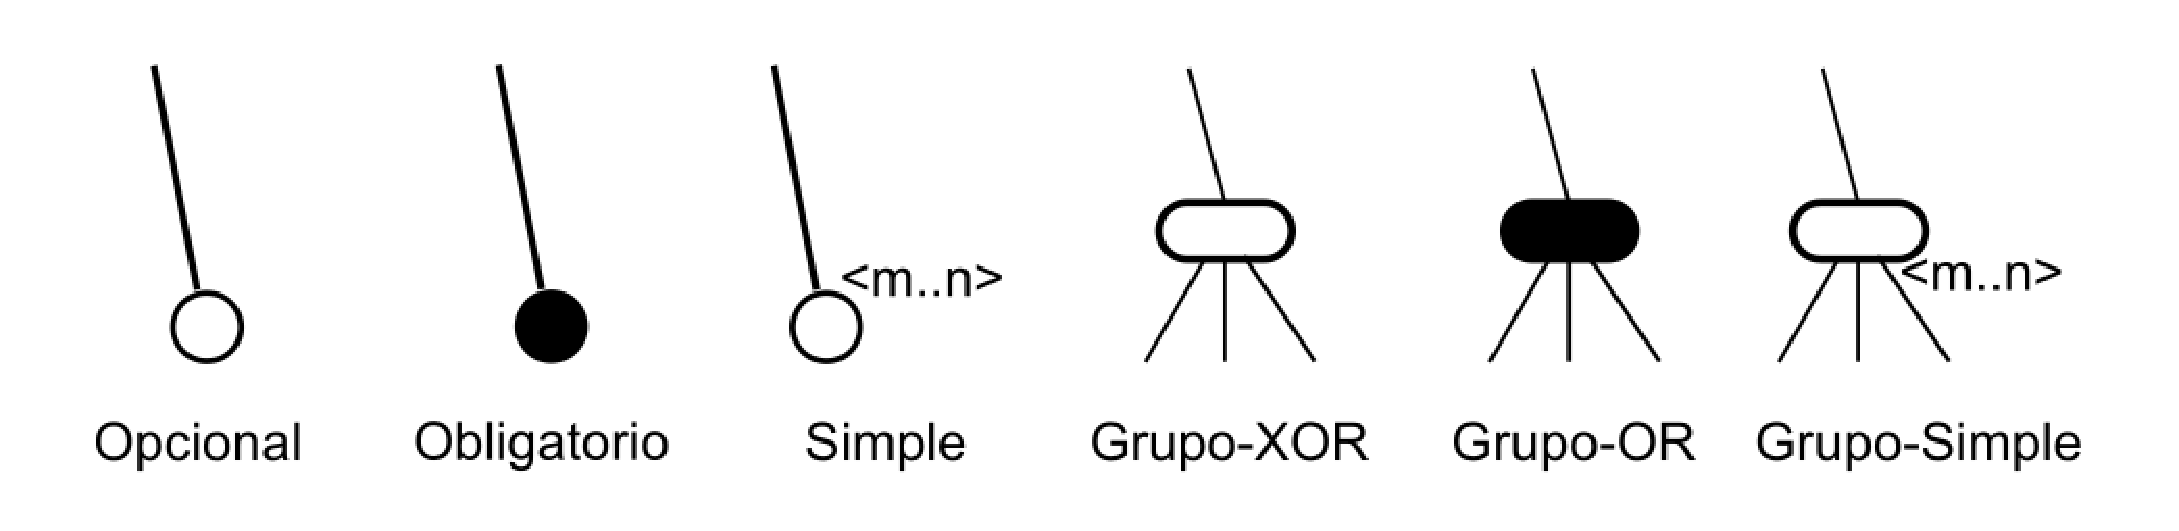
\includegraphics[scale=0.35]{background/relations.eps}
    \caption{Tipos de relaciones entre caracter�sticas }
    \label{fig:relacionesFeatures}
\end{figure}

A modo de resumen, la Figura~\ref{fig:relacionesFeatures} muestra las posibles relaciones que pueden entre caracter�sticas, as� como su representaci�n gr�fica. Dichas relaciones se describen a continuaci�n:

\begin{description}
    \item[Opcional] La caracter�stica hija puede estar o no estar seleccionada
    \item[Obligatoria] La caracter�stica siempre debe estar seleccionada.
    \item[Clonable] La caracter�stica tendr� una cardinalidad $<m,n>$, siendo m y n n�meros enteros que denotan el m�nimo y el m�ximo respectivamente de caracter�sticas que podemos seleccionar.
    \item[Grupo-xor] S�lo una de las caracter�sticas pertenecientes al grupo puede ser seleccionada.
    \item[Grupo-or] Debemos seleccionar como m�nimo una de las subcaracter�sticas, pudiendo seleccionar m�s si lo deseamos.
    \item[Grupo con cardinalidad] El n�mero m�nimo y m�ximo de caracter�sticas a seleccionar dentro del grupo vendr� determinado por su cardinalidad $<m,n>$.
\end{description}

Tras esta secci�n se han proporcionado al lector lo necesario para comprender el contexto del problema que este Proyecto Fin de Carrera pretende resolver. Las siguientes secciones est�n destinadas a explicar las tecnolog�as concretas que se han utilizado para implementar el lenguaje que da soluci�n a los problemas planteados. 


\section{\emph{Eclipse Modelling Framework}}
\label{sec:back:ecore}
%%==================================================================%%
%% Author : Tejedo Gonz�lez, Daniel                                 %%
%%          S�nchez Barreiro, Pablo                                 %%
%% Version: 1.0, 18/11/2012                                         %%                  
%%                                                                  %%
%% Memoria del Proyecto Fin de Carrera                              %%
%% Antecedentes, ecore                                              %%
%%==================================================================%%

EMF \emph{Eclipse Modeling Framework}~\cite{} es un \emph{plug-in} para Eclipse~\cite{} que permite elaborar metamodelos. Pera ello proporciona un lenguaje de metamodelo denominado Ecore, el cual se ha convertido en el est�ndar de factor para la realizaci�n de metamodelos. Utilizando Ecore se pueden crear metamodelos de forma gr�fica usando una notaci�n muy similar a la los diagramas de clases de UML. La Figura~\ref{fig:sle:metamodeloGrafo} muestra un sencillo ejemplo de metamodelo en Ecore (ver Secci�n~\ref{sec:intr:sle} para m�s detalles). EMF tambi�n incorpora una herramienta para la validaci�n reglas adicionales que no puedan ser especificadas a nivel de del metamodelo. 
 
EMF permite que, a partir de un metamodelo especificado en Ecore, podamos, utilizando diversos generadores de c�digo, crear autom�ticamente un conjunto de clases que nos permiten manipular dichos modelos a nivel de c�digo. Dichas clases se pueden adem�s distribuir como \emph{plug-in} para el entorno Eclipse.

Adem�s, al haberse convertido en est�ndar \emph{de facto} para el desarrollo de metamodelos, Ecore es compatible con multitud de herramientas para Ingenier�a de Lenguajes Dirigida por Modelos, como EMFText, la cual se describe en la siguiente secci�n, o diversos generadores de c�digo o herramientas de transformaci�n de modelos. 



\section{EMFText}
\label{sec:back:emftext}
%%==================================================================%%
%% Author : Tejedo Gonz�lez, Daniel                                 %%
%%          S�nchez Barreiro, Pablo                                 %%
%% Version: 1.0, 18/11/2012                                         %%
%% Version: 2.0, 06/02/2013                                         %%
%%                                                                  %%
%% Memoria del Proyecto Fin de Carrera                              %%
%% Antecedentes, emftext                                            %%
%%==================================================================%%


EMFText~\cite{} es una herramienta para dise�ar sintaxis textuales para metamodelos Ecore, siguiendo un enfoque de Ingenier�a de Lenguajes Dirigida por Modelos. Utilizando EMFText podemos definir la sintaxis textual de un lenguaje software utilizando una notaci�n similar a las de las notaci�n BNF. La Figura~\ref{fig:sle:gramaticaGrafos} muestra un ejemplo de gram�tica definida en EMFText para el lenguaje de grafos presentado en la Secci�n~\ref{sec:intr:sle}. 

%%==================================================================%%
%% NOTA(Pablo): Aqu� haz una gram�tica en EMFText para el lenguaje  %%
%%              de grafos del Cap�tulo 1                            %%
%%==================================================================%%

\begin{figure}[!tb]
    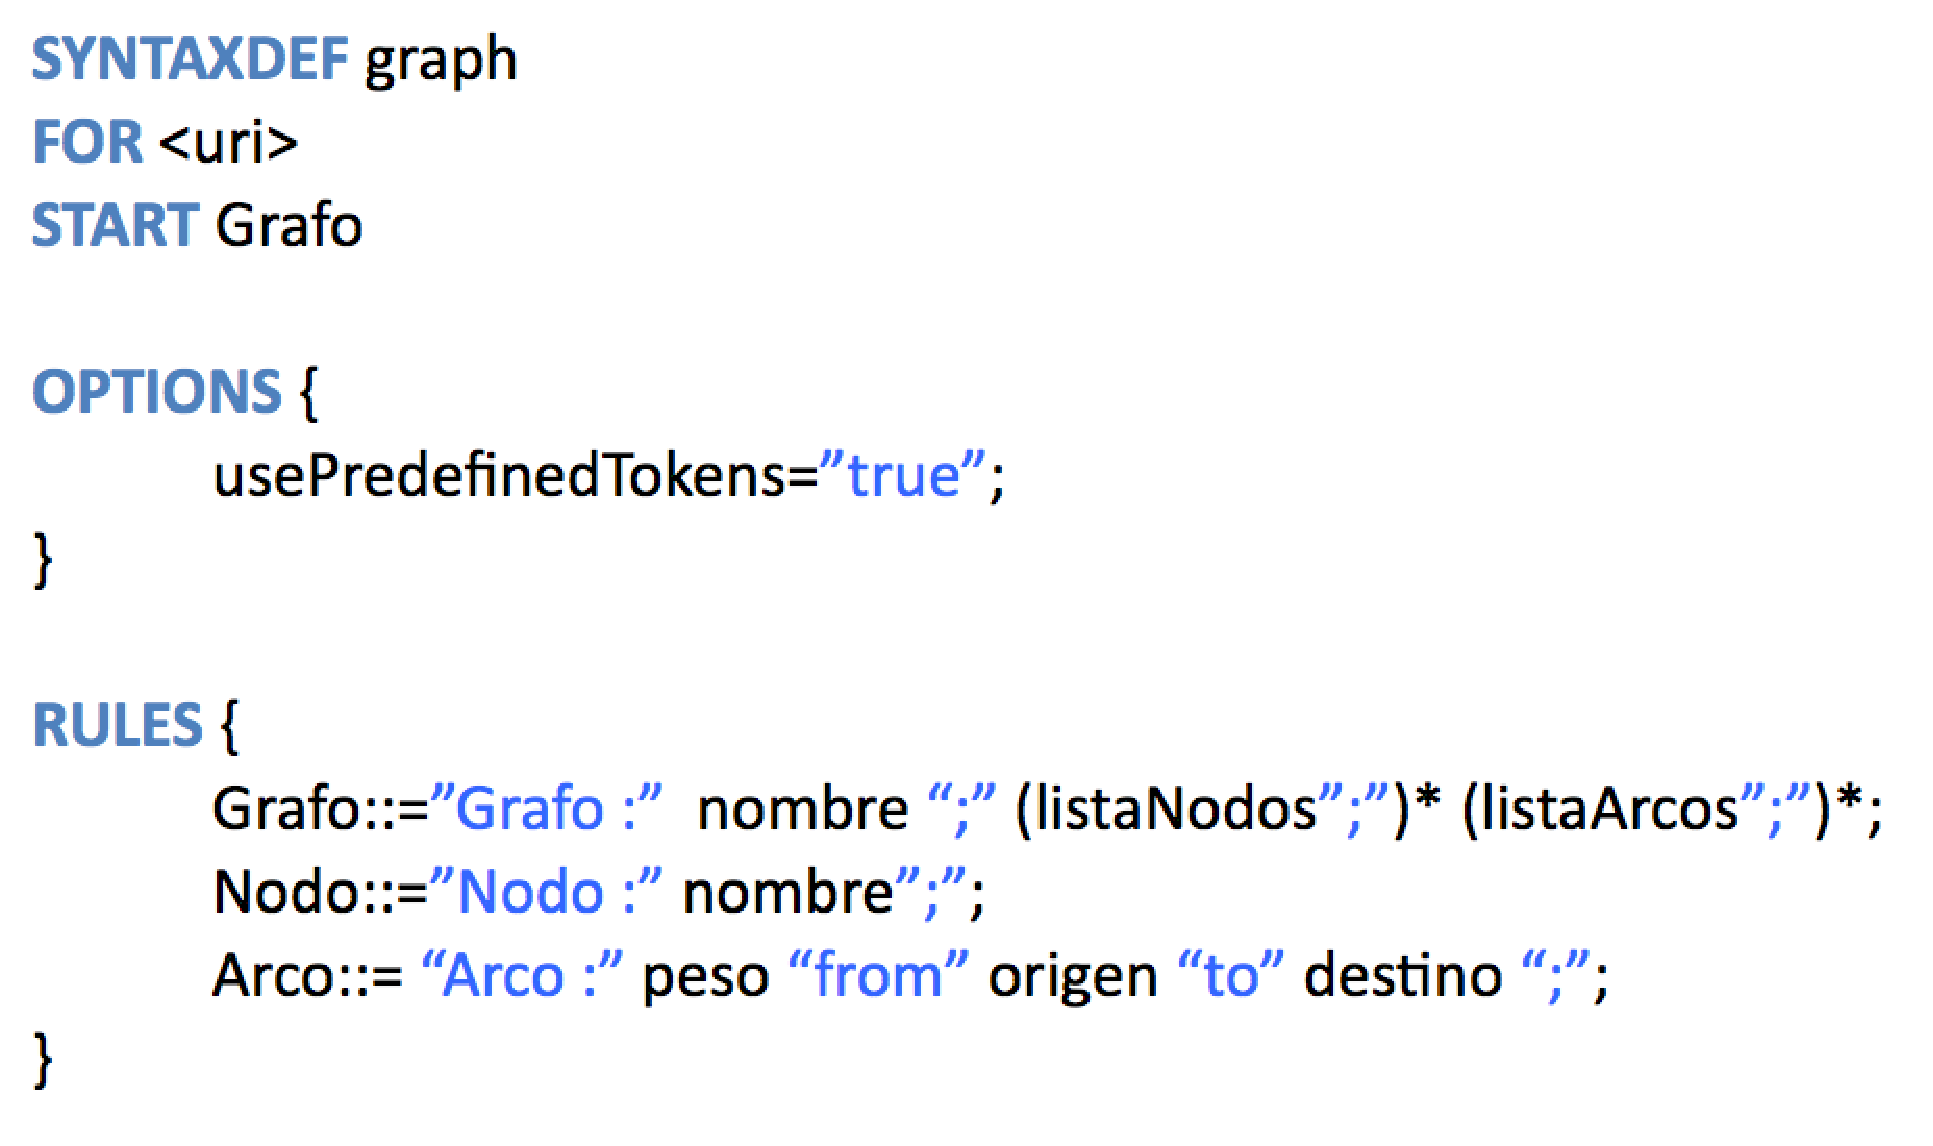
\includegraphics[scale=0.25]{background/gramaticaGrafo.eps}
    \caption{Gram�tica para el ejemplo del lenguaje de los grafos}
    \label{fig:sle:gramaticaGrafos}
\end{figure}

La sintaxis de EMFText difiere de las sintaxis BNF en que existen una serie de directivas para asociar elementos de la sintaxis textual con metaclases, de forma que se generen instancias de dichas metaclases a medida que se procesa el c�digo de un modelo. Por ejemplo, tal y como est� definida la gram�tica de la Figura~\ref{fig:sle:gramaticaGrafos}, a medida que vamos definiendo los arcos estamos indicando la informaci�n tanto de su peso como de sus nodos origen y destino. De este modo, EMFText genera una instanciaci�n de la metaclase Arco que inicializa con los datos le�dos y la a�ade a la instancia global del metamodelo.

La gran ventaja de EMFText es permite generar, a partir de la definici�n de una gram�tica, una gran cantidad de c�digo, liberando al programador de tareas tediosas que adem�s en muchos casos podr�an resultar complicadas. Utilizando EMFText se puede generar autom�ticamente: (1) un editor para nuestro lenguaje, con facilidades como coloreado de la sintaxis o autocompletado; (2) un procesador para el lenguaje capaz de generar una instancia de su correspondiente metamodelo; y (3) el c�digo necesario para empaquetar y distribuir dicho editor como un \emph{plug-in} para Eclipse. Adem�s, todo el c�digo generado es completamente independiente de EMFText, por lo que puede ser ejecutado en plataformas que no tengan instalado dicha herramienta; y es personalizable. Por ejemplo, se puede modificar f�cilmente el postprocesador de nuestra gram�tica. 






\section{Arquitectura de plugins de Eclipse}
\label{sec:back:eplugins}
%%==================================================================%%
%% Author : Tejedo Gonz�lez, Daniel                                 %%
%%          S�nchez Barreiro, Pablo                                 %%
%% Version: 1.0, 18/11/2012                                         %%                   
%% Version: 1.0, 06/02/2013                                         %%                   
%%                                                                  %%
%% Memoria del Proyecto Fin de Carrera                              %%
%% Antecedentes, arquitectura de plugins de eclipse                 %%
%%==================================================================%%

El entorno de desarrollo Eclipse es un ejemplo de arquitectura modular f�cilmente extensible mediante una compleja, pero sencilla al programador, arquitectura de \emph{plug-ins}. Un \emph{plug-in} en Eclipse es un componente que provee un cierto tipo de servicio dentro del contexto del espacio de trabajo de Eclipse. Es decir, una herramienta que se puede integrar en el entorno Eclipse junto con sus otras funcionalidades. Dado que la herramienta \emph{Hydra} fue dise�ada como un \emph{plug-in} para Eclipse, y nuestro editor pretende integrarse tanto en \emph{Hydra} como en \emph{Eclipse}, es necesario conocer y manejar el funcionamiento de la arquitectura de plug-ins de Eclipse.

Aunque la arquitectura de plug-ins de Eclipse tiene mucha profundidad y ofrece muchas posibilidades, es imprescindible el dominio de dos de sus conceptos clave para poder trabajar con ella: las dependencias y los puntos de extensi�n.  Mediante las dependencias podemos indicar que el plug-in a desarrollar tiene que incorporar toda la funcionalidad y estructura de otro plug-in (en este caso nuestro editor tiene, entre otras, una dependencia con el plug-in de la herramienta Hydra original). Un punto de extensi�n permite a�adir cierta funcionalidad al plug-in desarrollado mediante la inclusi�n autom�tica de ciertos segmentos de c�digo. Un ejemplo cl�sico de punto de extensi�n, y que adem�s ha sido utilizado en el transcurso de este proyecto, es el que permite a�adir un bot�n a la barra de tareas de Eclipse de manera autom�tica, teniendo que implementar �nicamente el c�digo del manejador de ese bot�n.

 \begin{figure}[!tb]
    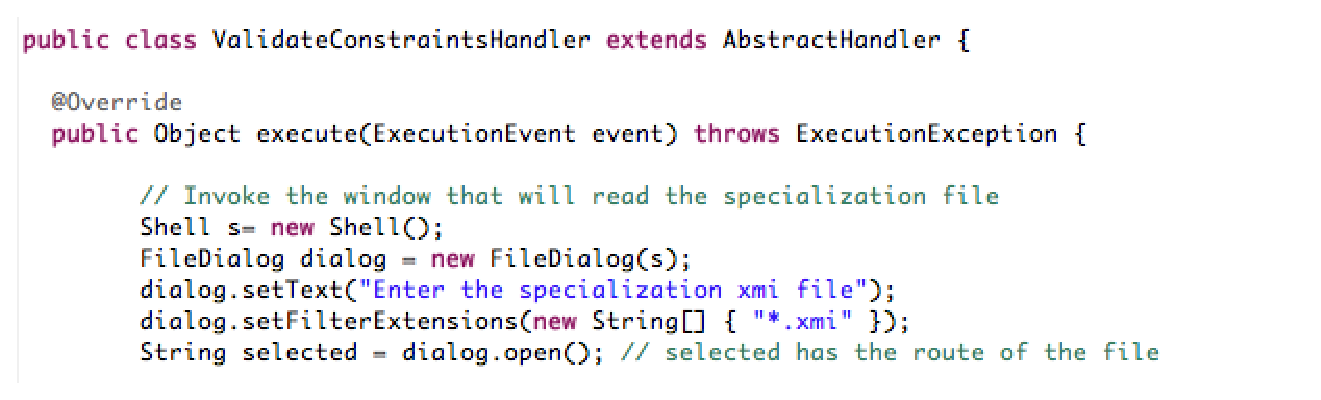
\includegraphics[scale=0.4]{background/codigoManejador.eps}
    \caption{Trozo de c�digo del manejador de un bot�n introducido mediante un punto de extensi�n}
    \label{fig:codigoManejador}
\end{figure}

%%==============================================================================================%%
%% NOTA(Pablo): Esto no se entiende nada
%%==============================================================================================%%
%%
%% En particular, se han utilizado mucho los puntos de extensi�n. Un punto de extensi�n en un
%% plug-in indica la posibilidad de que ese plug-in sea a su vez parte de otro, o que haya 
%% otros plug-ins que sean parte de �l. Esta particularidad permite no s�lo la integraci�n de 
%% nuestro editor con Hydra, sino tambi�n la personalizaci�n de men�s y botones para �l 
%% gracias a la creaci�n de puntos de extensi�n con plug-ins de creaci�n de men�s y barras de
%% herramientas.
%%
%%==============================================================================================%%

%%==============================================================================================%%
%% NOTA(Pablo): Para solucionar
%% - Describir en uno o dos p�rrafos c�mo funciona la arquietctura de plug-ins para Eclipse
%% - Poner un ejemplo de punto de extensi�n, sencillo y concreto, y explicar como funciona 
%%   el punto de extensi�n utilizando algo de c�digo.
%% Si no sabes como escribir esta secci�n, la eliminas directamente, y actualizas la intro 
%% al Cap�tulo de forma conveniente.
%%==============================================================================================%%


\section{Sumario}
\label{sec:back:sumario}
%===================================================================%%
%% Author : Tejedo Gonz�lez, Daniel                                 %%
%%          S�nchez Barreiro, Pablo                                 %%
%% Version: 1.0, 7/02/2013                                       %%                   
%%                                                                  %%
%% Memoria del Proyecto Fin de Carrera                              %%
%% Antecedentes, Sumario                      %%
%%==================================================================%%

Durante el cap�tulo de antecendes se han descrito los conceptos necesarios para lograr comprender el �mbito y el alcance de este proyecto, as� como el caso de estudio que se utilizar� a lo largo del documento en numerosas ocasiones y las tecnolog�as implicadas en el desarrollo de la aplicaci�n.
En el siguiente cap�tulo profundizaremos acerca del primer paso de la creaci�n de nuestro lenguaje de restricciones: la creaci�n de la sintaxis abstracta. Hablaremos con cierto nivel de detalle sobre el proceso de dise�o del metamodelo del lenguaje y sobre sus implicaciones.
